\section{Controller block}
This section will describe in detail how the controller block receives a target position and from it generates a duty cycle and direction based on the feedback.

\subsection{Description}

As mentioned before, the goal of this block is to regulate the motors in order to reach a desired position accurately. This can be done by implementing a closed loop controller. This controller was implemented as two separate components, a comparator component that generates the error used by a \textbf{PI} controller component to generate a duty cycle related to the error. By making a customized controller and a separate comparator component, it was also easier to implement some features, like ‘shortest path’, which will be discussed later on. 
Apart from the reasoning given by the control theory section, another reason to use a PI controller is that it is fairly easy to implement since the math required is simply gain and integration.


\subsection{Mathematical techniques}

This section will describe the theories used for the implementation.


\subsubsection{Discrete Integration}

Integration in discrete time is done by continuously sampling on a signal and relating the samples to each other. The technique used creates the square according to the previous error since this is arguably easier than other techniques to implement and that at a fast sampling rate the better precision gotten by using another technique is negligible. The method can be seen illustrated on figure \ref{fig:Integration_v1}.
The equation for the method can be derived to the following: Y = Y0 + X0t. Where Y is the output, Y0 is the previous output, X0 is the previous sampled value and t is the time between each sample. This equation only makes sense in the context that it is seen as a process that is run each time you take a new sample.


\begin{figure}[h!]
\centering
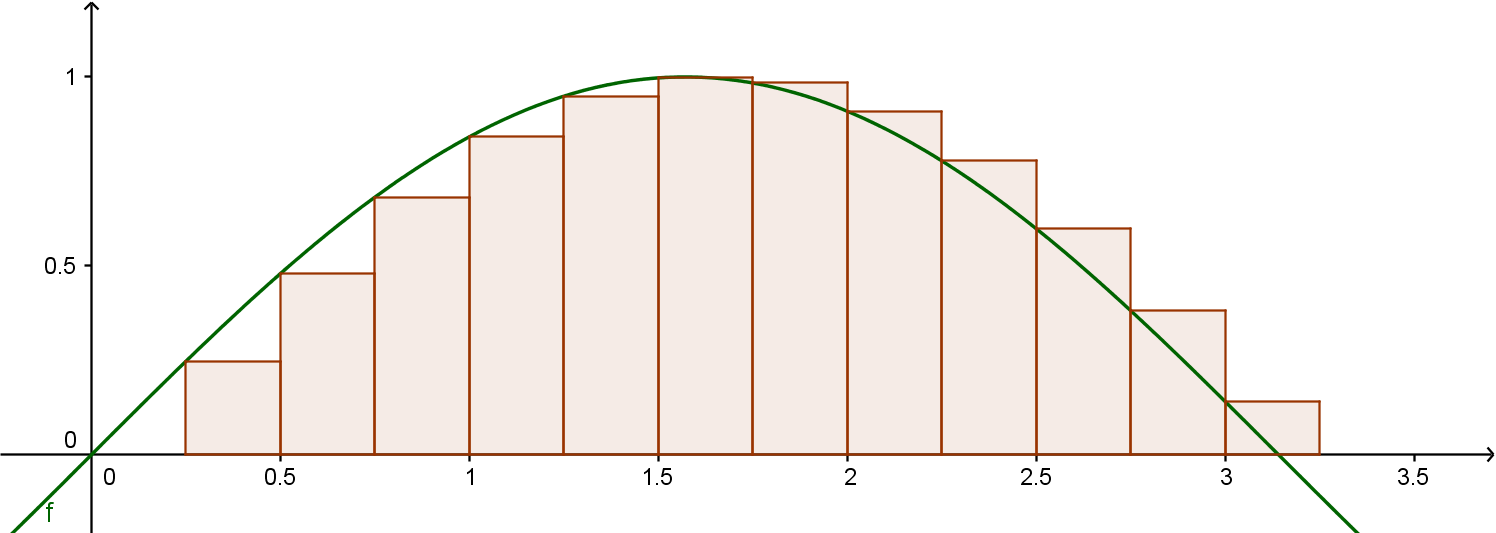
\includegraphics[scale=0.4]{Billeder/FPGA/Integration_v1.png}
\caption{Example of how integration is done.}
\label{fig:Integration_v1}
\end{figure}


\subsubsection{Shortest path}

Since the tilt part of the pan and tilt system is not restrained by wires, it is capable of turning more than 360 degrees. This means that the position can be related to that of a circle. However the control system sees this as straight line. This results in the control system being unable to go through the point of 0 if this is desired. The reason this happens is because a normal comparator is comparing the two values as if they were on a line instead of on a circle. So instead of making a normal comparator, a comparator that is capable of comparing values on a circle has to be made.
In order to make such a comparator, an analysis of the differences between values on a line and values on a circle is made. The first difference is that on a line there is only one way to a point, however there are always two ways on a circle. A notable observation is that the directions on the circle will always be opposite of each other.  The second difference, which is more like a similarity, is that one of the ways on the circle will always be equivalent to that of the line. The last thing to notice about the circle is that the distance is finite and since we know of the equivalence similarity, it can be derived that the distance of the other way has to be that of the equivalent part subtracted from circumference of the circle. It is also known that the direction of the other way has to be the opposite of that of the equivalent part. In conclusion, it is possible to make a comparator working in circles by applying some basic mathematics to the result of a normal comparator. Comparing the length of the two ways will determine the shortest path. An illustration of the two ways you can go on the circle can be seen on figure \ref{fig:Shortest_Comp_Short_and_Long}.


\begin{figure}[h!]
\centering
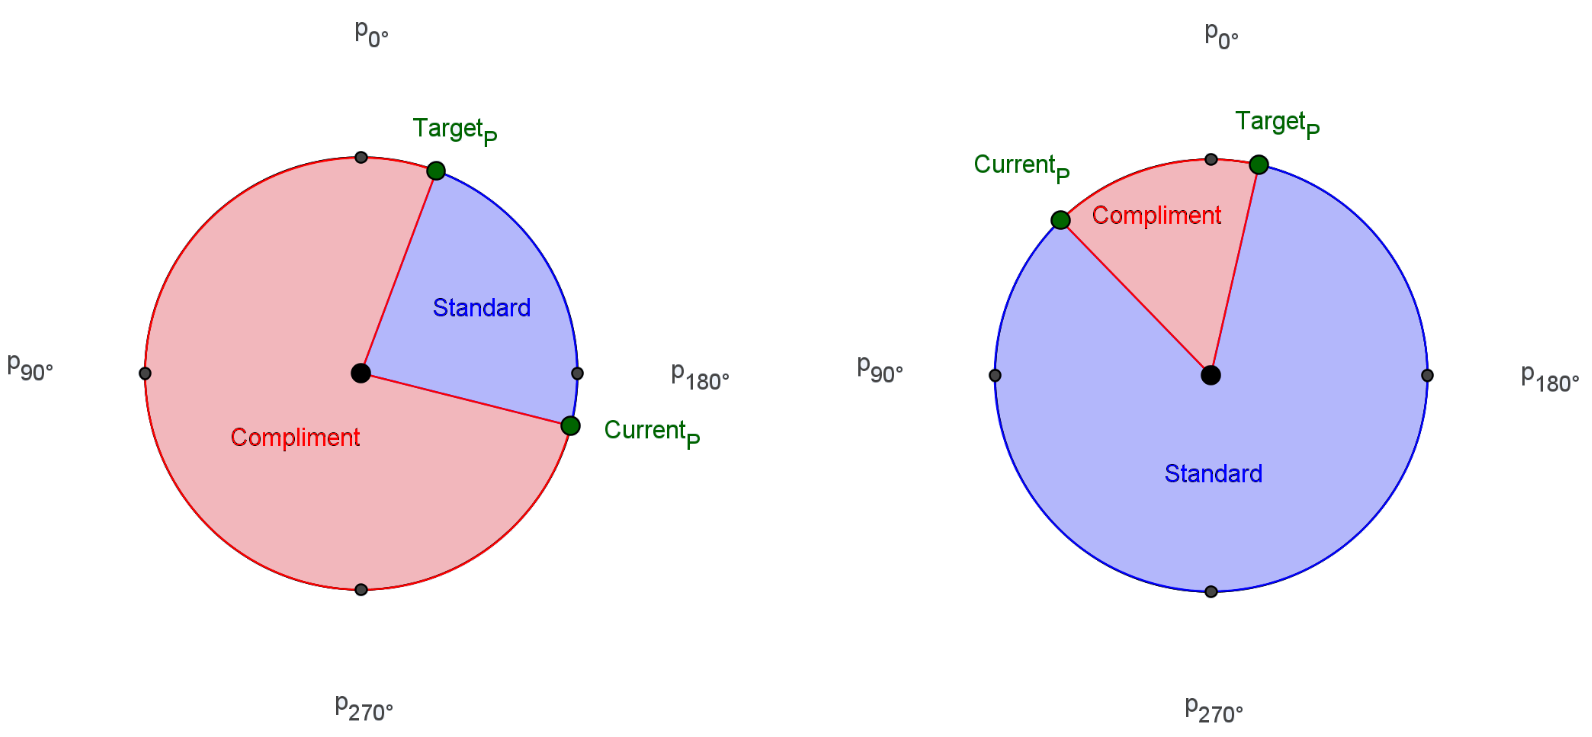
\includegraphics[scale=0.4]{Billeder/FPGA/Shortest_Comp_Short_and_Long.png}
\caption{Illustration of how the shortest path is found.}
\label{fig:Shortest_Comp_Short_and_Long}
\end{figure}


\subsection{Implementation}

The implementation will be explained by looking at the comparator and the PI controller separately. The reason this can be done is that the only connection these two have is the error produced by the comparator.


\subsubsection{Comparator}

The comparator receives the target position from the SPI slave and the feedback from the sensor, then starts by doing a normal comparison. This is done in a way where no negative values are reached by looking at which of the two is the smaller and subtracting this from the larger one. The direction is then set according to this criteria as well. This comparison can be seen on picture \ref{fig:Comperator code exaple}.


\begin{figure}[h!]
\centering
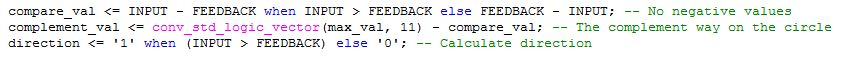
\includegraphics[scale=0.7]{Billeder/FPGA/Comperator_code_exaple.jpg}
\caption{Example of code from the comparator.}
\label{fig:Comperator code exaple}
\end{figure}


The next step for the comparator is to determine which direction on the circle leads to the shortest path between current and target position, which is accomplished by using aforementioned mathematics. The length of the shortest path is then sent to the PI controller as the error and the direction is send directly to the motor driver since the PI controller does not work in negative values, which will be discussed later.
Since the pan is restrained by the cables, a safety feature is needed to make sure that if the pan receives a position that contradicts this restraint, it does not move there. This was achieved using a position constraint in the comparator module. Note that since this is a base component that is shared by both the pan and tilt, it should be possible to turn off these constraints.



\subsubsection{PI controller}

The PI controller can be separated into calculating the P part, calculating the I part and then adding them together. Calculating the P part is quite simple since it is just taking the error and multiplying it by the constant set in the controller. However the I part requires that a sampling process is running. Inside this process a sampling is made and the arithmetic for the integration is done afterwards. The mathematics for the integration is simple enough to be implemented directly into code since t is a constant value. The sampling rate for the system was chosen to be 100kHz since this makes the error in the integration insignificant. The integration process can be seen on picture \ref{fig:PI controller code example}. Note that the division of t happens outside the process, since putting it in the process would make the value stay 0 because VHDL as a standard does not work in decimal and would just see values under zero, as zero. The summation is straightforward since it just requires P and I to be added. This concludes the controller part of the component, however there are still some practical restrictions that need to be added in order for the controller to work properly.


\begin{figure}[h!]
\centering
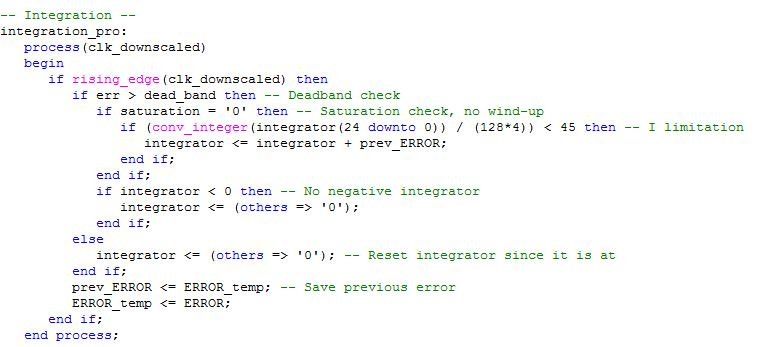
\includegraphics[scale=0.7]{Billeder/FPGA/PI_controller_code_example.jpg}
\caption{Example of the code from the PI controller.}
\label{fig:PI controller code example}
\end{figure}


One of the restrictions needed is the output format. Since the motor driver component requires a duty cycle represented as a value between 0 - 255 (8 bits), an upper limit for the output value is set. If the controller creates a value above this limit, the output is simply set to the limit, ensuring no data loss from overflowing the 8 bits.
To make the integrator more stable, anti wind-up was implemented. This was done by making the integrator halt the integration if the output is in saturation. This can be seen on the if statement checking for the saturation flag on picture \ref{fig:PI controller code example}. This ensures that the integrator is only running when the effect is needed.

Since the PI controller only works with positive values, this creates a problem where the integrator is only capable of increasing sum which essentially makes the system unstable. The best solution would always be to make the integrator integrate negatively. This would however require us to work in negative values. The integrator was implemented where it would reset upon having an error of 0. This is makes the controller less naturally close to the target position, however since we are tuning the PI controller not to overshoot, this less natural behaviour is negligible. Doing it this way would also take away some of the potential overshoot.
Upon testing the controller, it was noticed that integrator was reacting quite slowly, possibly because of the wind-up protection, which made it stop before reaching the destination and after a short time of standstill, the integrator would kick in, making the motor move the last bit. This could be solved simply by increasing the constant for the integrator part, however this would make it overshoot which was not desired. To solve this issue, a limit on the integrator part was implemented so that you would be able to increase the response of the integrator without the integrator making the system overshoot. The limit basically limited the speed the integrator part is contributing with.


\subsection{Tests}

The components have been tested separately because of the same reason stated before. The comparator tests were mainly done through simulation via. a testbench in the Xilinx IDE and the PI controller test were done on the pan and tilt system.


\subsubsection{Comparator}

The comparator was tested for different values which resulted in table \ref{fig:Comparator_test_table}, showing the tested values, the expected result and the actual result.


\begin{figure}[h!]
\centering
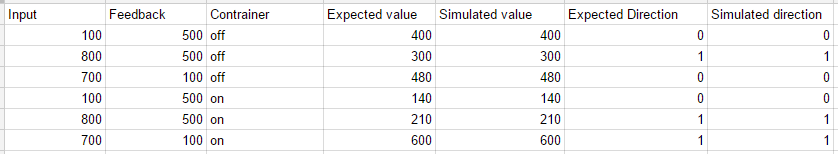
\includegraphics[scale=0.8]{Billeder/FPGA/Comparator_test_table.png}
\caption{Comparator test table.}
\label{fig:Comparator_test_table}
\end{figure}


\subsubsection{PI controller}

The PI controller were tested manually on the pan and tilt system. This test was done after the other components were tested working. A video of the test can be seen on Appendix \ref{sec:ContentonCD}.

\subsection{Discussion}

Some of the practical solutions in the PI controller have the consequence that the PI controller does not entirely follow control theory. Some of these problems would be not be there if the controller worked with negative values and since later in the development stage it was discovered that implementing the controller as a filter would have been optimal solution, these problems would not exist.


\subsection{Conclusion}

The components work as expected and the controller regulates as desired.